\documentclass[tikz,border=2pt]{standalone}
\usepackage{amsmath}
\usepackage{pgfplots}
\pgfplotsset{compat=1.18}
\usepgfplotslibrary{fillbetween}
\usetikzlibrary{arrows.meta}
\begin{document}
% X ~ N(2, 3^2). Left: density; dnorm(3, 2, 3) = 0.126 is the height at x = 3 and the shaded area
% left of 3 is pnorm(3, 2, 3) = 0.631. Right: the CDF (values from R's pnorm); pnorm goes from
% x = 3 to 0.631, qnorm goes from 0.95 back to x = 6.93.
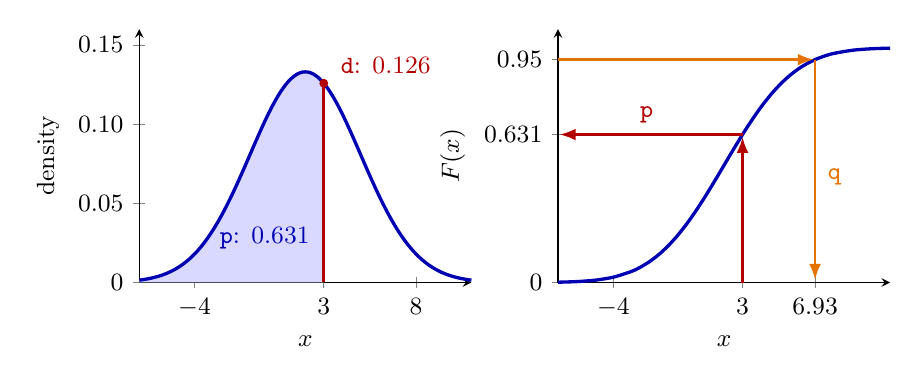
\begin{tikzpicture}[font=\small, >={Latex[length=2mm]}]
  \begin{axis}[name=dens, width=5.8cm, height=4.8cm, axis lines=left, xmin=-7, xmax=11, ymin=0, ymax=0.16,
      xtick={-4,3,8}, ytick={0,0.05,0.1,0.15}, yticklabels={0,0.05,0.10,0.15},
      xlabel={$x$}, ylabel={density}, tick label style={font=\small}, label style={font=\small},
      scaled y ticks=false, clip=false]
    \addplot[name path=f, blue!70!black, very thick, domain=-7:11, samples=121] {exp(-(x-2)^2/18)/(3*sqrt(2*pi))};
    \path[name path=base] (axis cs:-7,0) -- (axis cs:11,0);
    \addplot[blue!15] fill between[of=f and base, soft clip={domain=-7:3}];
    \draw[red!70!black, very thick] (axis cs:3,0) -- (axis cs:3,0.12579);
    \fill[red!70!black] (axis cs:3,0.12579) circle (1.6pt);
    \node[red!70!black, anchor=west] at (axis cs:3.4,0.137) {\texttt{d}: $0.126$};
    \node[blue!70!black] at (axis cs:-0.2,0.028) {\texttt{p}: $0.631$};
  \end{axis}
  \begin{axis}[at={(dens.east)}, anchor=west, xshift=1.1cm, width=5.8cm, height=4.8cm, axis lines=left,
      xmin=-7, xmax=11, ymin=0, ymax=1.08, xtick={-4,3,6.93}, xticklabels={$-4$,$3$,$6.93$},
      ytick={0,0.631,0.95}, yticklabels={0,0.631,0.95},
      xlabel={$x$}, ylabel={$F(x)$}, tick label style={font=\small}, label style={font=\small}, clip=false]
    \addplot[blue!70!black, very thick, smooth] coordinates {(-7,0.0013) (-6,0.0038) (-5,0.0098) (-4,0.0228) (-3,0.0478) (-2.5,0.0668) (-2,0.0912) (-1.5,0.1217) (-1,0.1587) (-0.5,0.2023) (0,0.2525) (0.5,0.3085) (1,0.3694) (1.5,0.4338) (2,0.5) (2.5,0.5662) (3,0.6306) (3.5,0.6915) (4,0.7475) (4.5,0.7977) (5,0.8413) (5.5,0.8783) (6,0.9088) (6.5,0.9332) (7,0.9522) (7.5,0.9666) (8,0.9772) (9,0.9902) (10,0.9962) (11,0.9987)};
    \draw[->, red!70!black, thick] (axis cs:3,0) -- (axis cs:3,0.62);
    \draw[->, red!70!black, thick] (axis cs:3,0.6306) -- (axis cs:-6.9,0.6306);
    \node[red!70!black, anchor=south] at (axis cs:-2.2,0.64) {\texttt{p}};
    \draw[->, orange!90!black, thick] (axis cs:-7,0.95) -- (axis cs:6.85,0.95);
    \draw[->, orange!90!black, thick] (axis cs:6.93,0.95) -- (axis cs:6.93,0.012);
    \node[orange!90!black, anchor=west] at (axis cs:7.1,0.45) {\texttt{q}};
  \end{axis}
\end{tikzpicture}
\end{document}
